\chapter{Metodologia do trabalho}
\label{CAP3}

Esta seção trata das fases do trabalho: como deverão ser executadas e em que sequência.

% descrever fases do trab: concepcao, projeto, implementacao, testes
% (falar com o prof)


\section{Coleta de dados via OBD-II e pelo celular}
Já existe uma plataforma aceleradora desenvolvida no GitHub que consegue comunicar-se com o veículo através do protocolo OBD-II\textsuperscript{[12]}. Esse outro projeto implementa o protocolo OBD-II e também uma interface gráfica básica para mostrar os dados fornecidos pelo carro.

A figura \ref{fig:git_obd_interface} mostra uma plataforma onde é possível ver alguns dos dados já previstos.

\begin{figure}[hp]
    \centering
    
    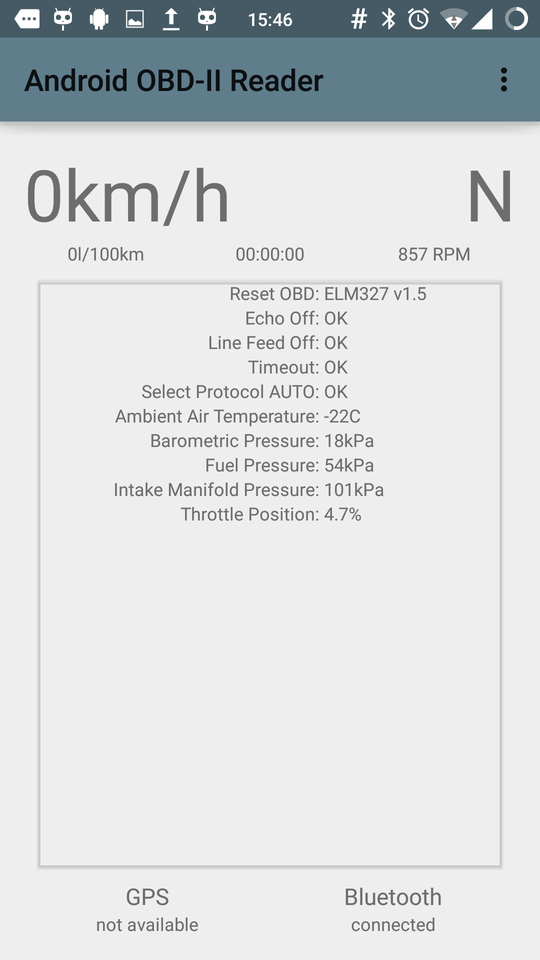
\includegraphics[scale=0.3]{figures/git_obd_interface.png}
    
    \caption{Interface básica com porta OBD-II\textsuperscript{[12]}.}
    
    \label{fig:git_obd_interface}
\end{figure}

Nesta fase do desenvolvimento caracteriza-se pela adaptação do aplicativo para que possa atender aos requisitos do projeto.

Primeiro, será preciso entender a estrutura e o funcionamento do código através da IDE do \textit{Android Studio}, que foi por onde essa plataforma foi originalmente desenvolvida.

Complementarmente ao que for fornecido pela porta OBD, poderão ser usados também dados externos ao carro, como os de navegação fornecidos pelo Waze através dos próprios motoristas que passam em cada via\textsuperscript{[13]}, informações de localização via GPS e também a aceleração desempenhada pelo carro durante seu trajeto.

Essas outras informações serão de grande importância na fase final do projeto, de análise dos dados coletados.

A viabilidade dessa última parte, de utilizar dados fornecidos pelo celular, pode ser vista em um estudo publicado em 2014 no \textit{site} da IEEXplore\textsuperscript{[15]}.

Esse artigo utiliza parâmetros de movimentos bruscos do carro, p.ex. mudança de faixa, e a velocidade do veículo para classificar o motorista como mais ou menos agressivo, a partir de um \textit{score} chamado de \textit{driver safety index}.

A figura \ref{fig:sudden_acc_car} ilustra como essa análise pode ser feita, mas sem entrar em detalhes técnicos de como isso é possível.

\begin{figure}[hp]
    \centering
    
    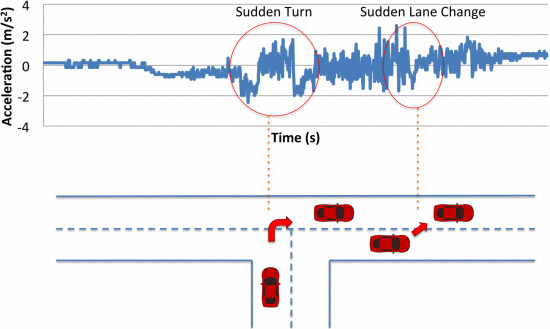
\includegraphics[scale=0.6]{figures/sudden_acc_car.jpg}
    
    \caption{Correspondência entre variações de aceleração e movimentos relativos do carro\textsuperscript{[15]}.}
    
    \label{fig:sudden_acc_car}
\end{figure}

\section{Transferência de dados para a nuvem e estruturação}
Uma vez que a plataforma aceleradora esteja adaptada ao novo sistema, os dados coletados deverão ser passados para uma plataforma remota, que armazenará os dados brutos coletados para depois serem processados e analisados na fase seguinte.

O \textit{pipeline} de captura e armazenamento de informações estará consolidado quando for definida uma estrutura fixa para o processamento dos dados crus e o formato em que serão guardados na nuvem.

Isso poderá ser feito fixando-se uma especificação básica de arquivos JSON que deverá ser seguida pelas APIs que fizerem uso do banco de dados da nuvem.

\section{Geração dos dados}
O sistema poderá ser usado assim que os protocolos e estruturas básicos de comunicação tiverem sido definidos. 

Neste momento serão necessários voluntários para fornecer dados ao sistema e quanto mais pessoas puderem participar, melhor será a análise de perfil feita ao fim do projeto.

\section{Visualização dos dados}
Uma aplicação Web básica para visualização dos dados individuais de cada motorista deverá ser implementada.

Essa plataforma deverá permitir que apenas usuários autorizados acessem suas próprias informações. Para isso, algum sistema de segurança deverá ser implementado.

Na área logada do motorista, será possível visualizar estatísticas básicas acerca do que foi coletado pela porta OBD.

A princípio, serão apresentados bem poucos dados, os quais serão definidos assim que o sistema for um pouco mais palpável. 

\section{Análise dos dados}
Finalmente, com toda a infraestrutura do projeto já funcional, será possível gerar estatísticas relevantes sobre cada motorista.

Quais parâmetros serão gerados ou que análise será feita objetivamente ainda será objeto de discussão no projeto, mas uma das ideias primárias era tentar definir métricas que diferenciem um motorista do outro, isto é, que definam o seu perfil de condução.

Conforme o artigo citado anteriormente (\textit{Driver behaviour profiling using smartphone sensory data in a V2I environment}\textsuperscript{[15]}), é possível usar métricas de movimentação brusca do carro para classificar motoristas segundo a segurança de sua direção.

Mais especificamente, o estudo determina quatro tipos de condutores: muito cautelosos, cautelosos, agressivos e muito agressivo\textsuperscript{[15]}.

A classificação depende basicamente de quantos movimentos bruscos são feitos e em que situações eles ocorrem. Isso significa que em um ponto de maior convergência de estradas, por exemplo, haverá maior penalidade para o \textit{driver safety index} que em um local de menos movimento ou.

Dessa forma, esse estudo procura ranquear melhor os motoristas que têm menos probabilidade de gerar acidentes.